\documentclass{article}[11pt]

\usepackage{natbib}
\usepackage[sc]{mathpazo}
\usepackage[T1]{fontenc}
\usepackage{amsmath}
\usepackage{amsfonts}
\usepackage{amssymb}
\usepackage{graphicx}
\usepackage[onehalfspacing]{setspace}
\usepackage{color}
\usepackage[margin=.75in, tmargin=0.71in, bmargin=0.71in]{geometry}
\usepackage{url}

\usepackage{appendix}
\usepackage{hyperref}
\usepackage{xcolor}
\usepackage{todonotes}
\usepackage{booktabs}
\usepackage{lscape}
\usepackage{caption}%
\usepackage{bbm}
\usepackage{comment}

\usepackage{longtable}

\usepackage{subcaption}

\usepackage{bookmark}

\usepackage{babel}
\usepackage[autostyle, english = american]{csquotes}
\MakeOuterQuote{"}

\title{Textual Analysis and Financial Statements}
\author{Isaac Liu}

\setlength{\parindent}{0pt}
\setlength{\parskip}{0.5em}

\hypersetup{
    colorlinks=true,
    linkcolor=black,
    filecolor=black,      
    urlcolor=blue,
    citecolor=black
}

% stattotex commands
\newcommand{\avgCompanyMentions}{97.78}
\renewcommand{\avgCompanyMentions}{98.66}
\renewcommand{\avgCompanyMentions}{98.66}

\newcommand{\numQuarters}{4724}
\newcommand{\numCompanies}{387}
\renewcommand{\numQuarters}{4724}
\renewcommand{\numCompanies}{387}
\renewcommand{\numQuarters}{4724}
\renewcommand{\numCompanies}{387}
\renewcommand{\numQuarters}{4724}
\renewcommand{\numCompanies}{387}
\renewcommand{\numQuarters}{4724}
\renewcommand{\numCompanies}{387}
\renewcommand{\numQuarters}{4724}
\renewcommand{\numCompanies}{387}
\renewcommand{\numQuarters}{4724}
\renewcommand{\numCompanies}{387}
\renewcommand{\numQuarters}{4724}
\renewcommand{\numCompanies}{387}
\renewcommand{\numQuarters}{4724}
\renewcommand{\numCompanies}{387}
\renewcommand{\numQuarters}{4724}
\renewcommand{\numCompanies}{387}
\renewcommand{\numQuarters}{4724}
\renewcommand{\numCompanies}{387}
\renewcommand{\numQuarters}{4724}
\renewcommand{\numCompanies}{387}
\renewcommand{\numQuarters}{4724}
\renewcommand{\numCompanies}{387}
\renewcommand{\numQuarters}{4724}
\renewcommand{\numCompanies}{387}
\renewcommand{\numQuarters}{4724}
\renewcommand{\numCompanies}{387}
\renewcommand{\numQuarters}{4,724}
\renewcommand{\numCompanies}{387}
\renewcommand{\numQuarters}{4,724}
\renewcommand{\numCompanies}{387}
\renewcommand{\numQuarters}{4,724}
\renewcommand{\numCompanies}{387}

\newcommand{\avgCallLength}{8,776.18}
\renewcommand{\avgCallLength}{8,754.25}
\renewcommand{\avgCallLength}{8,754.25}
\renewcommand{\avgCallLength}{8,759.68}
\renewcommand{\avgCallLength}{8,759.68}


\begin{document}

	\maketitle

    \section*{Introduction}

    Corporate credit ratings represent professional estimations of the default risk carried by company debt. These ratings represent critical information for investors - not just institutional investors and financially sophisticated bondholders, but also stockholders, who may be wiped out completely in the event of bankruptcy. Analyzing ways to predict ratings can offer substantial value to a variety of stakeholders. Predictive models may be useful for investors without access to data, companies or potential lenders that seek information about influential factors (there is evidence suggesting financial factors and projections have a causal impact on ratings and are not manipulated by companies in response to forecasted rating changes \citep{he_impact_2018}), and by any parties seeking interpolated ratings for companies that do not have them.

    In this project, we seek to fully leverage the text of earnings calls, along with traditional financial measures and variables, to improve predictions of corporate credit ratings for any given company and quarter and better understand the importance of various influences.\footnote{Though much literature has focused on financial statements and reports and credit ratings (as just one example, see \cite{makwana_understanding_2022}), our paper takes a relatively underexplored approach, instead incorporating earnings call transcripts. We believe calls offer a richer picture of a firm's financial prospects because they include two-way conversation between company management and financial analysts in form of a Q and A section. This section incorporates the broader beliefs and concerns of the financial community into our predictions. Additionally, in contrast to financial statements, which must be (noisily) parsed to identify sections relevant to management analysis, earnings calls provide more directly valuable and readily available information.} Textual features such as pre-trained language model vector embeddings \citep{araci_finbert_2019} and analyses of sentiment accompany tabular variables as inputs to a variety of supervised machine learning techniques for classification from logistic regression to tree-based methods. If time allows, we will also incorporate advances in the study of graph neural networks to create additional embeddings modelling linkages between firms \citep{das_credit_2023} implied by calls.

    To the best of our knowledge, the closest prior work to ours is \cite{donovan_measuring_2021}, which leverages the textual content of earnings calls and financial statements to predict credit events such as bankruptcies, interest spread changes, and rating downgrades using unigram and bigram frequencies and the supervised machine learning techniques of Support Vector Regression, Latent Dirichlet Allocation, and Random Forests. The coefficient on a constructed textual measure of credit risk was found to be significant up the 1\% level. In contrast to this approach, we focus on predicting the credit ratings themselves, and integrate more techniques from machine learning such as the power of pre-trained language models and a wider variety of algorithms for classification.

    \section*{Data and Exploratory Data Analysis}

    We combine a wide variety of data sources to support our predictions of credit ratings - merging rating data with company earnings calls, financial statement variables, and industry sector. In our final dataset, each observation represents a fixed quarter date (1/1, 4/1, 7/1, 10/1) for a company, with the company's most recent credit rating, earnings call and associated financial statement variables, and sector attached.

    Our scope of interest is publicly traded companies from 2010-2016 (a limitation due to the availability of credit rating data). The data is temporally unbalanced, with many companies entering the dataset in later years, after they first receive an observable credit rating (Figure \ref{fig:obs-by-quarter-year}).

    \begin{figure}[h!]
		\centering
        \caption{Observations by Quarter and Year}
        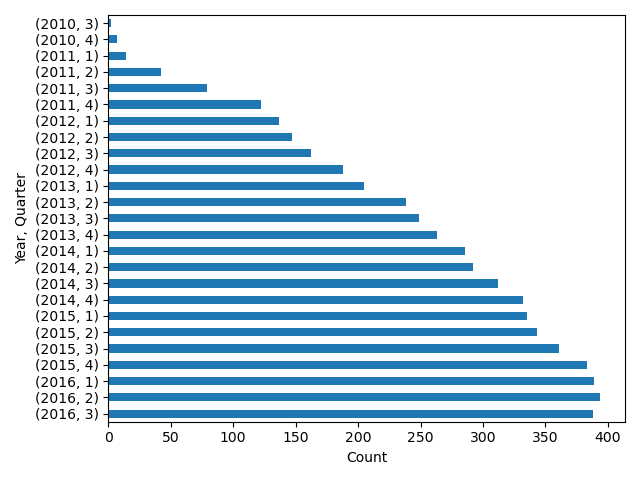
\includegraphics[width=0.5\linewidth,keepaspectratio=true]{../Output/All Data EDA/Tabular EDA/all_data_fixed_quarter_dates_obs_by_year_quarter_no_title.png}
        \label{fig:obs-by-quarter-year}
	\end{figure}

    To ensure comparability, we drop items missing any predictor variable. In all, we have \numQuarters \space quarters for \numCompanies \space unique companies.

    \subsection*{Credit Ratings}

    We make use of long-term credit rating issuances from S and P Rating Services, provided from a combination of two credit rating datasets downloaded in CSV and Excel format from Kaggle \citep{gewerc_corporate_2020,makwana_corporate_2022}. Each issuance be a change in rating (upgrade, downgrade) or reaffirmation - they occur at ad-hoc intervals. We reshape these rating issuances to a dataset of ratings for each company on each fixed quarter date by creating a rating end date variable that is the date of the next issuance, and joining a list of the fixed quarter dates on the condition that the fixed quarter date is between the issuance date and the end date.

    Figure \ref{fig:credit-ratings} shows the distribution of rating grades used in our final dataset. Finer grades (+, -) are sometimes assigned by agencies, but these grades were removed for this project. Ratings of BBB and above are considered investment grade - these bonds carry empirical one-year default rates of ~0 to 1\%. Ratings below that are classified as junk, with default rates from 1 to 30, 40, or even 50\% for some years \citep{s_and_p_global_ratings_s_2024}. Most company-quarters have ratings around the BBB threshold, with very few cases on the extreme ends of the spectrum.

    \begin{figure}[h!]
		\centering
        \caption{Credit Ratings}
        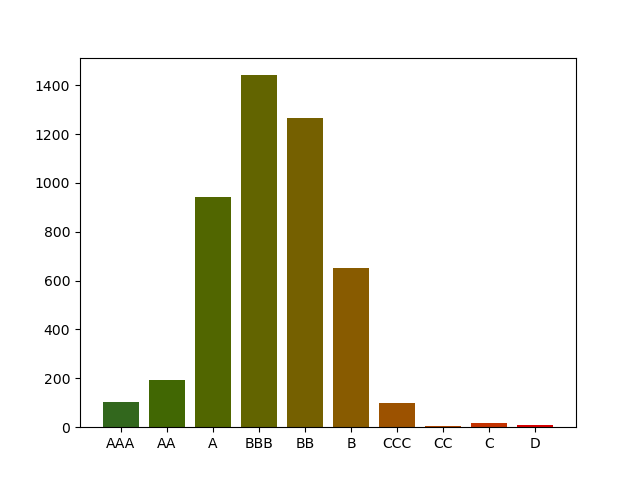
\includegraphics[width=0.5\linewidth,keepaspectratio=true]{../Output/All Data EDA/Tabular EDA/Distribution of Rating Issuances_no_title.png}
        \label{fig:credit-ratings}
	\end{figure}

    \subsection*{Earnings Calls}

    Our earnings call data comes from the Financial Modelling Prep API \citep{financial_modeling_prep_financial_2024}, a trusted source widely used in industry. We remove all calls that happened more than 250 days prior and after the year and quarter they are supposed to discuss the results from. Including both prepared remarks and analyst Q and A sessions, the overall average call length in our final data stands at \avgCallLength \space words.

    \begin{figure}[h!]
		\centering
        \caption{Number of Words in Earnings Calls}
        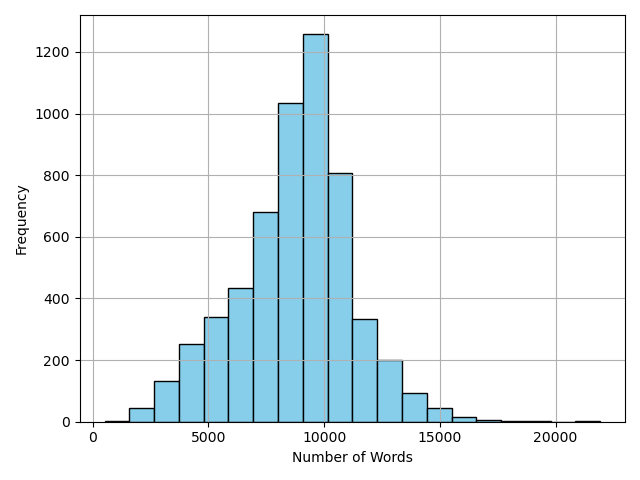
\includegraphics[width=0.5\linewidth,keepaspectratio=true]{../Output/All Data EDA/NLP EDA/all_data_num_words_distribution_no_title.png}
	\end{figure}

    \subsection*{Financial Statements}

    Our financial statement variables are also retrieved using the Financial Modelling Prep API. We make use of items from company balance sheets, cash flow statements, and income statements, as well as company market capitalization. We include 124 variables in total, such as revenue, total liabilities, net income, EBITDA.
    
    To prepare the data, we limit our observations to items reported in USD, check for and correct items off by a factor of 1,000 as a result of parsing (if last few digits are 000.00 and the item is above or below 2.5\% and 97.5\% quantile, divide by 1,000), and check some accounting identities in \cite{das_credit_2023}, setting failing variables to missing. We also discard observations where statement filing dates do not agree between the three types of statements, where the filing date falls outside of the fixed quarter matched on via earnings call date, and where the filing date is more than 45 days after the earnings call date.

    In some of our models, we make use of Altman's Z-score, a traditional measure of bankruptcy risk that accounts for company earnings, equity, and assets and liabilities \citep{altman_financial_1968} (for details on the construction of the score, see Appendix section \ref{sec:altman-z-score}). Figure \ref{fig:altman-z-score} shows the distribution of adjusted Z-scores in our dataset. Though interpretations of the score vary, traditionally, values above 3.0 have been considered safe, while those below 1.8 are considered to have a high chance of bankruptcy. Though such an interpretation is potentially overly pessimistic for our data, we do have some companies on both ends of the spectrum.

    \begin{figure}[h!]
		\centering
        \caption{Altman Z-Score}
        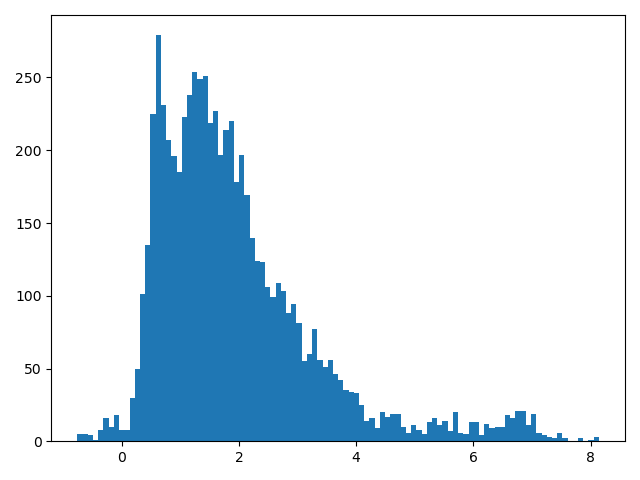
\includegraphics[width=0.5\linewidth,keepaspectratio=true]{../Output/All Data EDA/Tabular EDA/altman_z_score_all_data_no_title.png}
        \label{fig:altman-z-score}
	\end{figure}    

    \subsection*{Sector}

    The GCIS industry classification standard divides companies into 11 major industry sectors (there are finer groupings as well, but this data was not easily obtainable for our project) \citep{s_and_p_gics_2024}. It is widely used in the financial community, and was developed in part by S and P, the same company responsible for our credit ratings. We obtained classifications from Kaggle in CSV format and supplemented them with manual lookup \citep{kozlov_us_2022}. Figure \ref{fig:firms-by-sector} shows the unfortunate sectoral imbalance present in our data, with a large share of firms in consumer, industrial, and technology sectors, relative to very few in the distinctly different financials and real estate sectors.

    \begin{figure}[h!]
		\centering
        \caption{Firms by Sector}
        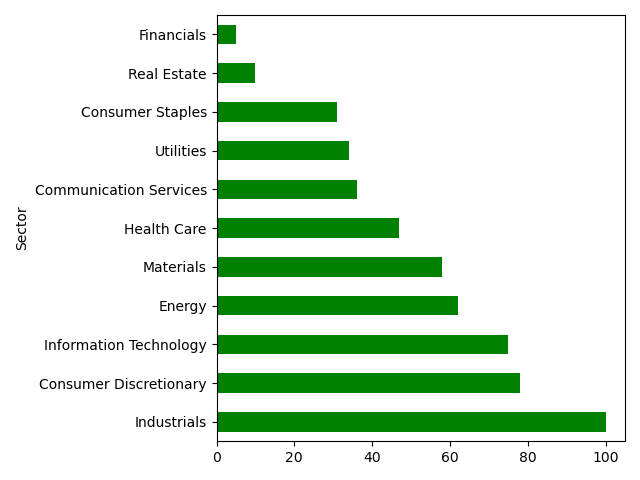
\includegraphics[width=0.5\linewidth,keepaspectratio=true]{../Output/All Data EDA/Tabular EDA/all_data_fixed_quarter_dates_firms_by_sector_no_title.png}
        \label{fig:firms-by-sector}
	\end{figure}

    \subsection*{Quality Control}

    Our data preparation was subject to rigorous quality control standards. We extensively code reviewed all data cleaning code. Our exploratory analyses identified data quality issues such as extreme values in financial statement variables, which we handled by winsorizing, and date gaps between quarters, earnings calls, and financial statements, which we dropped in the case of aggregiously mismatched observations. We carefully removed companies that only provided annual reporting. We also removed all observations for Peabody Energy (ticker BTU), the only company in our dataset to declare bankruptcy (April 13, 2016) due to substantial concern about missing data leading up to the event.

    \section*{NLP Features}

    In general, average call length in words appears to be positively correlated with credit rating, with the companies with the highest ratings having the longest calls, as shown in Figure \ref{fig:call-length-by-credit-rating}.
    
    \begin{figure}[h!]
		\centering
        \caption{Average Call Length by Credit Rating}
        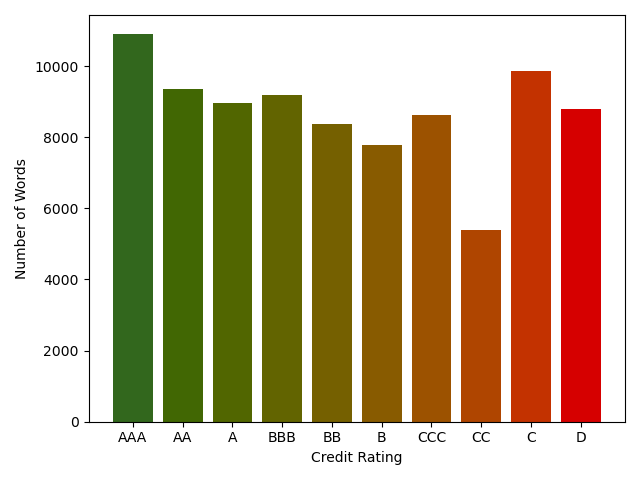
\includegraphics[width=0.5\linewidth,keepaspectratio=true]{../Output/All Data EDA/NLP EDA/all_data_call_length_by_credit_rating_no_title.png}
        \label{fig:call-length-by-credit-rating}
	\end{figure}

    We have prepared both FinBERT\footnote{BERT is a pretrained transformer-based language model that encodes text into embedding vectors using surrounding context. FinBERT is a version of BERT finetuned for tasks in the financial domain (language model embedding performance can vary greatly by domain).} \citep{araci_finbert_2019} and Doc2Vec\footnote{This method involves constructing representations of each call based on the bag-of-words and skipgram tasks - a neural network is trained to either a word or a word's context while accounting for a vector identifying the document.} \citep{le_distributed_2014} embeddings to represent each call, and are considering using these as inputs to our classifier.

    \section*{Modelling}

    Our overall model architecture is of the form

    \begin{equation*}
        \text{Predicted Credit Rating} = f(\text{Financial Statement Variables}, \text{Sector}, \text{NLP Features})
    \end{equation*}

    Our first model is a simple logistic regression

    XXX logistic regression predictors

    multinomial, balanced class weights, l1 penalty

    variable importance

    table of predictions

    fitting and output

    assumptions
    
    interpretation

    \section*{Conclusion and Next Steps}

    We have seen above that textual and NLP features are contributing to our predictions...

    One major next step is continuing to improve the construction of our NLP features and methods. Much more work could be done to improve the construction of our sentiment scores and analysis - seeking out better pretrained models for earnings call sentiment, or improving the methods through which embedding representations are converted to sentiment. Some members of the group have also been working on a separate class project involving annotating earnings calls with topics discussed. This work could be integrated into our project to provide additional features for our models - we could identity topics and then connect them to credit ratings. Finally, we could try building an end-to-end transformer classifier that takes in earnings calls and outputs credit ratings (perhaps finetuning and adding a classifier on top of the longformer \citep{beltagy_longformer_2020} transformer encoder model (suitable for document, rather than word or sentence embedding creation)).

    We've also begun using the AutoML library Autogluon to explore a wider variety of classifiers. Autogluon runs a wide variety of state-of-the-art prediction algorithms and performs hyperparameter tuning. The results, shown in Table \ref{tab:autogluon-leaderboard} for all allowed predictors in our dataset (metadata about call and statement dates, the rating on the previous fixed quarter date, all the financial statement variables, all the constructed NLP features, and sector) can provide a good starting point for our further modelling choices.

    \begin{table*}
        \centering
        \caption{Autogluon Leaderboard}
        \begin{tabular}{lr}
\toprule
Model & Test Accuracy \\
\midrule
ExtraTreesGini & 0.929844 \\
XGBoost & 0.928731 \\
CatBoost & 0.928731 \\
LightGBM & 0.927617 \\
LightGBMXT & 0.927617 \\
WeightedEnsembleL2 & 0.927617 \\
LightGBMLarge & 0.927617 \\
RandomForestEntr & 0.926503 \\
ExtraTreesEntr & 0.925390 \\
RandomForestGini & 0.925390 \\
NeuralNetTorch & 0.920935 \\
NeuralNetFastAI & 0.920935 \\
KNeighborsUnif & 0.250557 \\
KNeighborsDist & 0.247216 \\
\bottomrule
\end{tabular}

        \label{tab:autogluon-leaderboard}
    \end{table*}

    Tree-based bagging and boosting methods (boosting in particular) seem to perform extraordinarily well on our modelling task (ExtraTrees is a somewhat simplified variant of random forest; GBM stands for Gradient Boosting Machine). Each of the trained models also comes with a set of optimized hyperparameters - after selecting a model, we will further tune these hyperparameters to improve performance. The library also provides feature importance measures, computed by permuting each feature and measuring the drop in accuracy. Though these tests are not of high quality (and many results are not reported or are not significant), they confirm that previous ratings, earnings call word counts and tone variables, a few financial variables, and several date metadate variables are all very important.

    Another area of interest for us is continuing to pursue the approach in \cite{das_credit_2023}, which uses graph neural networks to model the relationships between companies in combination with tabular financial data and NLP features. Prerequisite to this approach is the construction of an undirected graph showing linkages between companies based on the earnings call data. 
    
    We've pursued begun work on this step from two angles. First, following the original paper, Doc2Vec embeddings representing calls can be averaged for each company. A graph can then be constructed with connecting edges added for cases when the vectors for each company have cosine similarity above a certain threshhold.

    As a second approach, which also opens more opportunities for exploration even without a neural network, we have used transformer-based Named Entity Recognition to identify mentions of any company in each earnings call. On average, each earnings call has \avgCompanyMentions \space company mentions - Figure \ref{fig:company-mentions} shows the distribution. Our next step involves the use of entity resolution algorithms (trigram matching, supervised learning) to link these mentions to firm tickers in order to construct a graph of relationships.

    \begin{figure}[h!]
		\centering
        \caption{Company Mentions}
        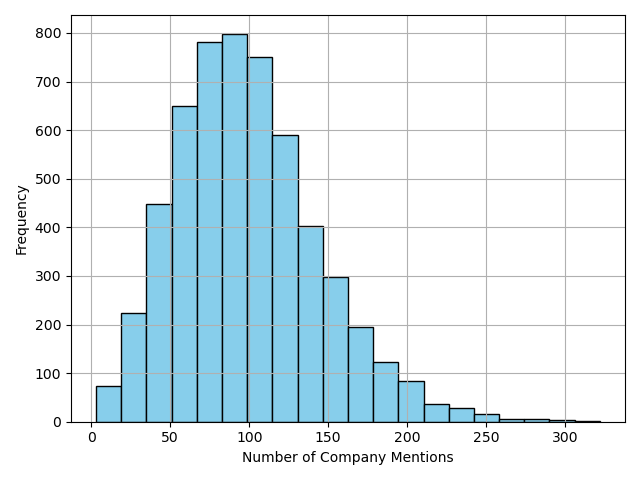
\includegraphics[width=0.5\linewidth,keepaspectratio=true]{../Output/All Data EDA/NLP EDA - NER on Company Names/Company Mentions Distribution No Title.png}
        \label{fig:company-mentions}
	\end{figure}
    
    \clearpage
    \newpage

    \bibliographystyle{aea}
    \bibliography{Stat-222-Capstone}

    \clearpage
    \newpage

    \appendix

    \section{Appendix}

    \subsection{Altman's Z-Score}

    \label{sec:altman-z-score}

    As in \cite{das_credit_2023}, the components of the Z-score are as follows:

    \begin{itemize}
        \item A: EBIT / Total Assets
        \item B: Net Sales / Total Assets
        \item C: Market Capitalization / Total Liabilities
        \item D: Working Capital / Total Assets
        \item E: Retained Earnings / Total Assets
    \end{itemize}

    We Winsorize extreme values of Ratio A, B, D, and E by setting the top and bottom 2.5\% of values to the 97.5 and 2.5 percentile, respectively. Due to the presence of additional outliers and the sourcing of market capitalization from a different dataset than the rest of the variables, Ratio C is instead Winsorized over the top and bottom 5\% of values. 

    The ratios are combined via the following equation:

    \begin{equation*}
        \text{Z-Score} = 3.3 A + 0.99 B + 0.6 C + 1.2 D + 1.4 E
    \end{equation*}

\end{document}
